%!TEX root = ../dokumentation.tex

\section{Klassendiagramm}

\begin{figure}[!htbp]
	\centering
	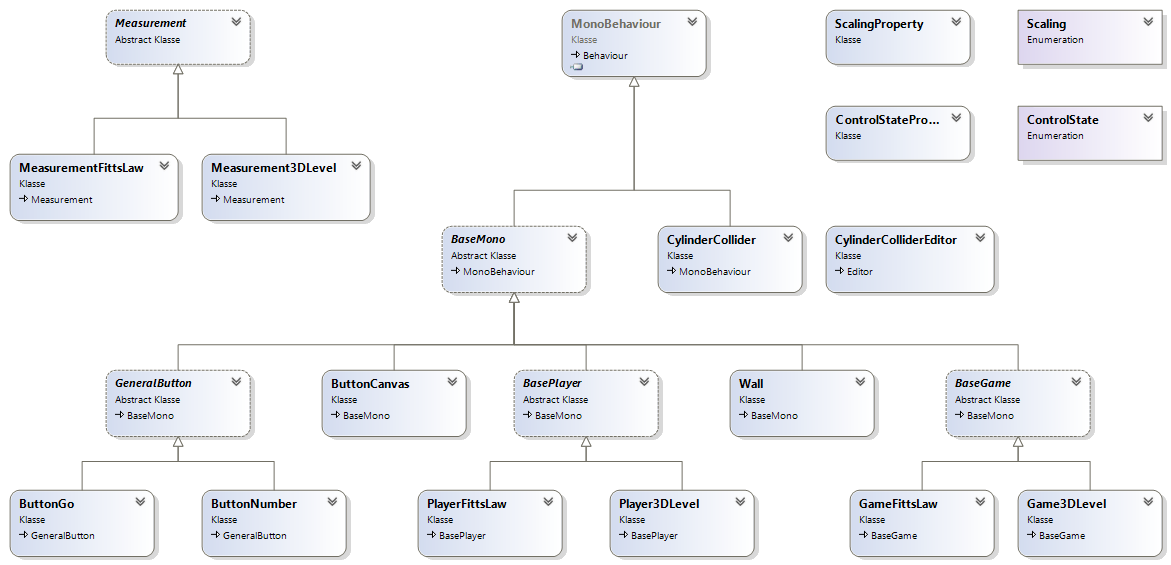
\includegraphics[angle=90,height=0.9\textheight]{ClassDiagram}
	\caption[Übersicht Klassenhierarchie]{Übersicht Klassenhierarchie}
	\label{fig:ClassDiagram}
\end{figure}

\section{Tabelle der Versuche}
% Please add the following required packages to your document preamble:
% \usepackage{booktabs}
% \usepackage{graphicx}

\begin{table}[H]	
	\caption{Tabelle der Versuche}
	\label{table:probanden}
	\resizebox{\textwidth}{!}{%
		\begin{tabular}{@{}lllll@{}}
			\toprule
			Proband & Laserpointer und Trigger & Laserpointer und Blinzeln & Eye-Tracking und Trigger & Eye-Tracking und Blinzeln \\ \midrule
			1  & (3, 2), (2, 2), (3, 3) & (3, 2), (1, 2), (3, 3) & (3, 4), (2, 4), (3, 2) & (2, 3), (1, 3), (2, 1) \\
			2  & (1, 3), (3, 3), (1, 4) & (2, 1), (1, 1), (2, 3) & (1, 3), (2, 3), (1, 2) & (3, 2), (1, 2), (3, 4) \\
			3  & (1, 4), (2, 4), (1, 3) & (1, 4), (3, 4), (1, 3) & (1, 1), (2, 1), (1, 3) & (1, 4), (2, 4), (1, 3) \\
			4  & (3, 4), (1, 4), (3, 1) & (2, 4), (3, 4), (2, 1) & (2, 3), (3, 3), (2, 2) & (1, 1), (3, 1), (1, 2) \\
			5  & (3, 1), (1, 1), (3, 3) & (2, 3), (3, 3), (2, 4) & (1, 3), (3, 3), (1, 2) & (3, 1), (1, 1), (3, 2) \\
			6  & (2, 2), (3, 2), (2, 3) & (3, 1), (2, 1), (3, 4) & (3, 2), (1, 2), (3, 1) & (2, 2), (3, 2), (2, 3) \\
			7  & (2, 1), (3, 1), (2, 4) & (2, 2), (3, 2), (2, 4) & (2, 4), (3, 4), (2, 2) & (3, 3), (2, 3), (3, 2) \\
			8  & (2, 4), (3, 4), (2, 3) & (2, 1), (3, 1), (2, 4) & (2, 3), (3, 3), (2, 4) & (3, 4), (1, 4), (3, 3) \\
			9  & (1, 1), (2, 1), (1, 4) & (1, 2), (2, 2), (1, 4) & (2, 1), (1, 1), (2, 2) & (1, 2), (2, 2), (1, 1) \\
			10 & (3, 1), (2, 1), (3, 3) & (1, 2), (3, 2), (1, 3) & (3, 1), (2, 1), (3, 3) & (2, 1), (1, 1), (2, 2) \\
			11 & (2, 1), (3, 1), (2, 4) & (3, 1), (1, 1), (3, 3) & (1, 4), (2, 4), (1, 2) & (2, 2), (3, 2), (2, 4) \\
			12 & (1, 4), (3, 4), (1, 1) & (1, 1), (3, 1), (1, 4) & (3, 4), (1, 4), (3, 1) & (2, 4), (3, 4), (2, 3) \\
			13 & (1, 2), (2, 2), (1, 1) & (2, 2), (1, 2), (2, 3) & (3, 1), (1, 1), (3, 2) & (1, 4), (3, 4), (1, 2) \\
			14 & (3, 2), (2, 2), (3, 4) & (2, 2), (3, 2), (2, 3) & (3, 4), (1, 4), (3, 2) & (3, 3), (1, 3), (3, 1) \\
			15 & (3, 3), (2, 3), (3, 2) & (1, 4), (3, 4), (1, 3) & (2, 1), (1, 1), (2, 2) & (2, 1), (3, 1), (2, 4) \\
			16 & (1, 3), (2, 3), (1, 2) & (1, 3), (3, 3), (1, 4) & (3, 4), (1, 4), (3, 1) & (2, 1), (3, 1), (2, 2) \\
			17 & (1, 2), (2, 2), (1, 1) & (2, 1), (1, 1), (2, 4) & (2, 2), (1, 2), (2, 3) & (1, 4), (2, 4), (1, 1) \\
			18 & (2, 4), (3, 4), (2, 1) & (3, 3), (1, 3), (3, 4) & (1, 3), (2, 3), (1, 1) & (1, 4), (3, 4), (1, 3) \\
			19 & (1, 2), (3, 2), (1, 3) & (2, 2), (1, 2), (2, 3) & (2, 4), (1, 4), (2, 1) & (1, 3), (3, 3), (1, 2) \\
			20 & (1, 3), (2, 3), (1, 2) & (3, 1), (1, 1), (3, 2) & (3, 3), (1, 3), (3, 2) & (2, 3), (3, 3), (2, 1) \\ \bottomrule
		\end{tabular}%
	}
\end{table}

\section{Eye-Tracking Heatmaps der Probandenversuche}
\label{appendix:heatmaps}
\begin{figure}[!htbp]
	\centering
	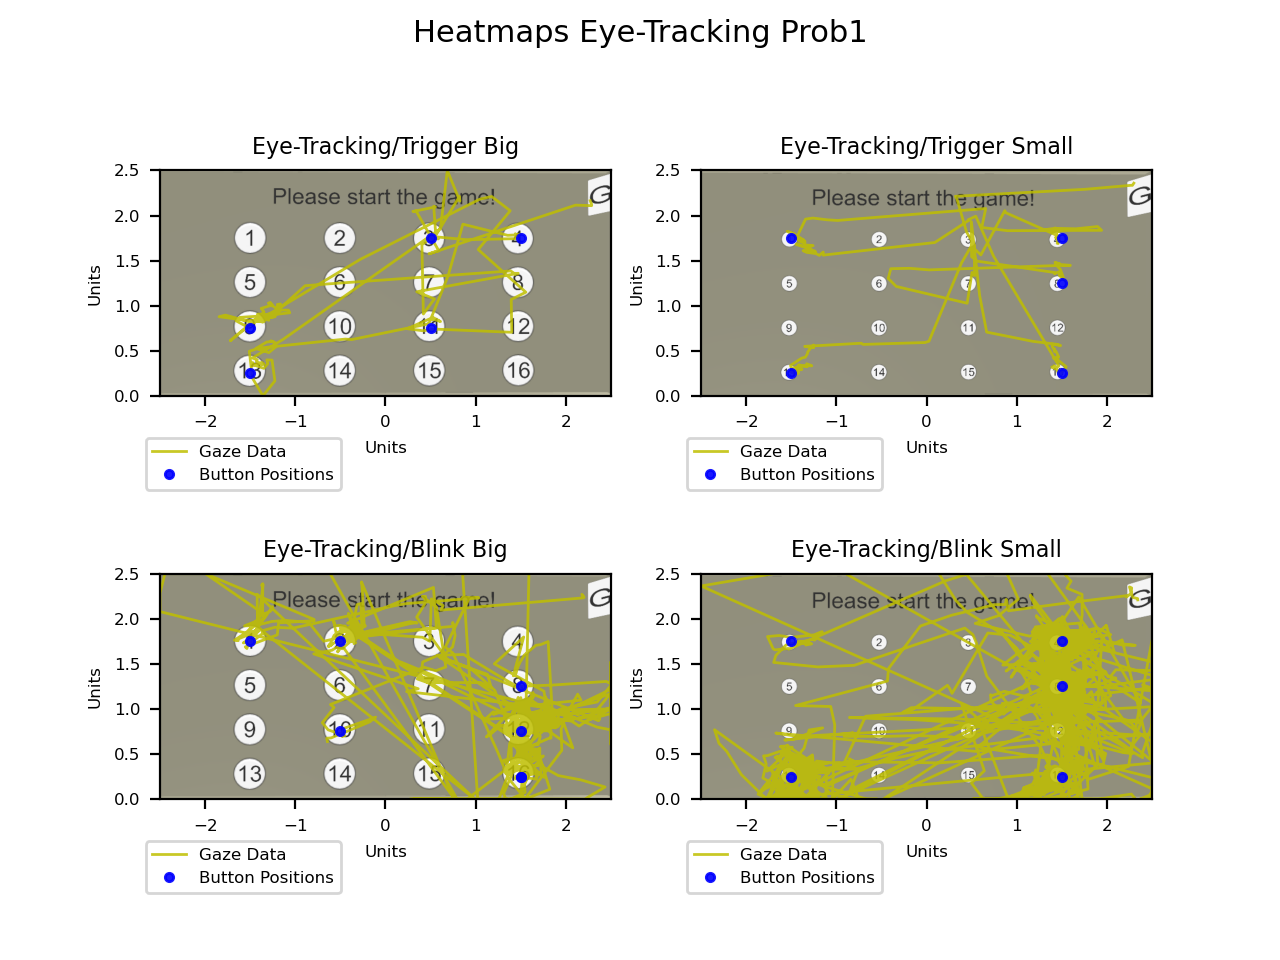
\includegraphics[width=1.0\linewidth]{plot_heatmap_prob1}
	\caption[Visualisierung der Blickdaten und der auszuwählenden Knöpfe] {Visualisierung der Blickdaten und der auszuwählenden Knöpfe}
\end{figure}
\begin{figure}[!htbp]
	\centering
	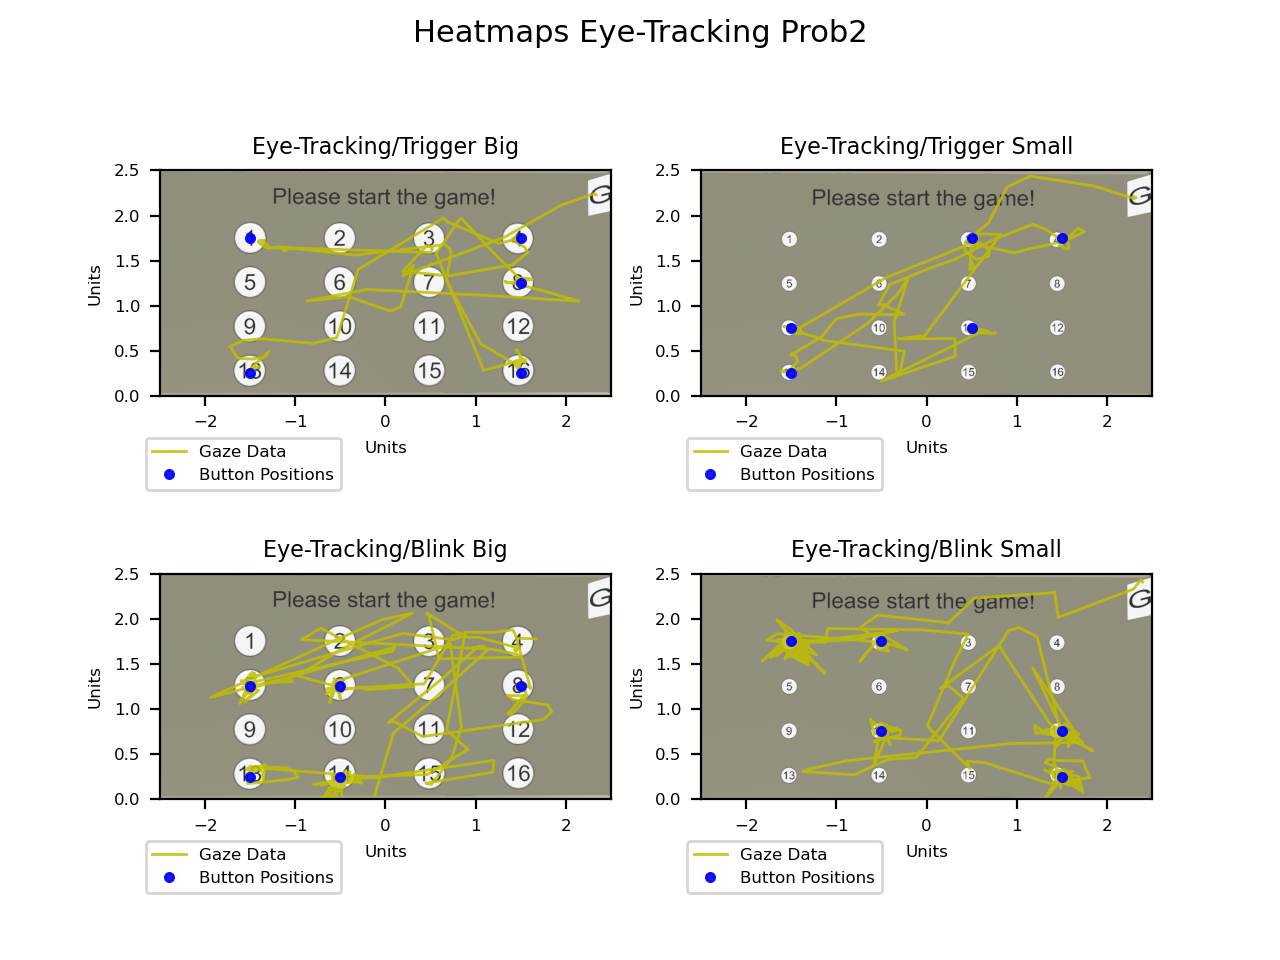
\includegraphics[width=1.0\linewidth]{plot_heatmap_prob2}
	\caption[Visualisierung der Blickdaten und der auszuwählenden Knöpfe] {Visualisierung der Blickdaten und der auszuwählenden Knöpfe}
\end{figure}
\begin{figure}[!htbp]
	\centering
	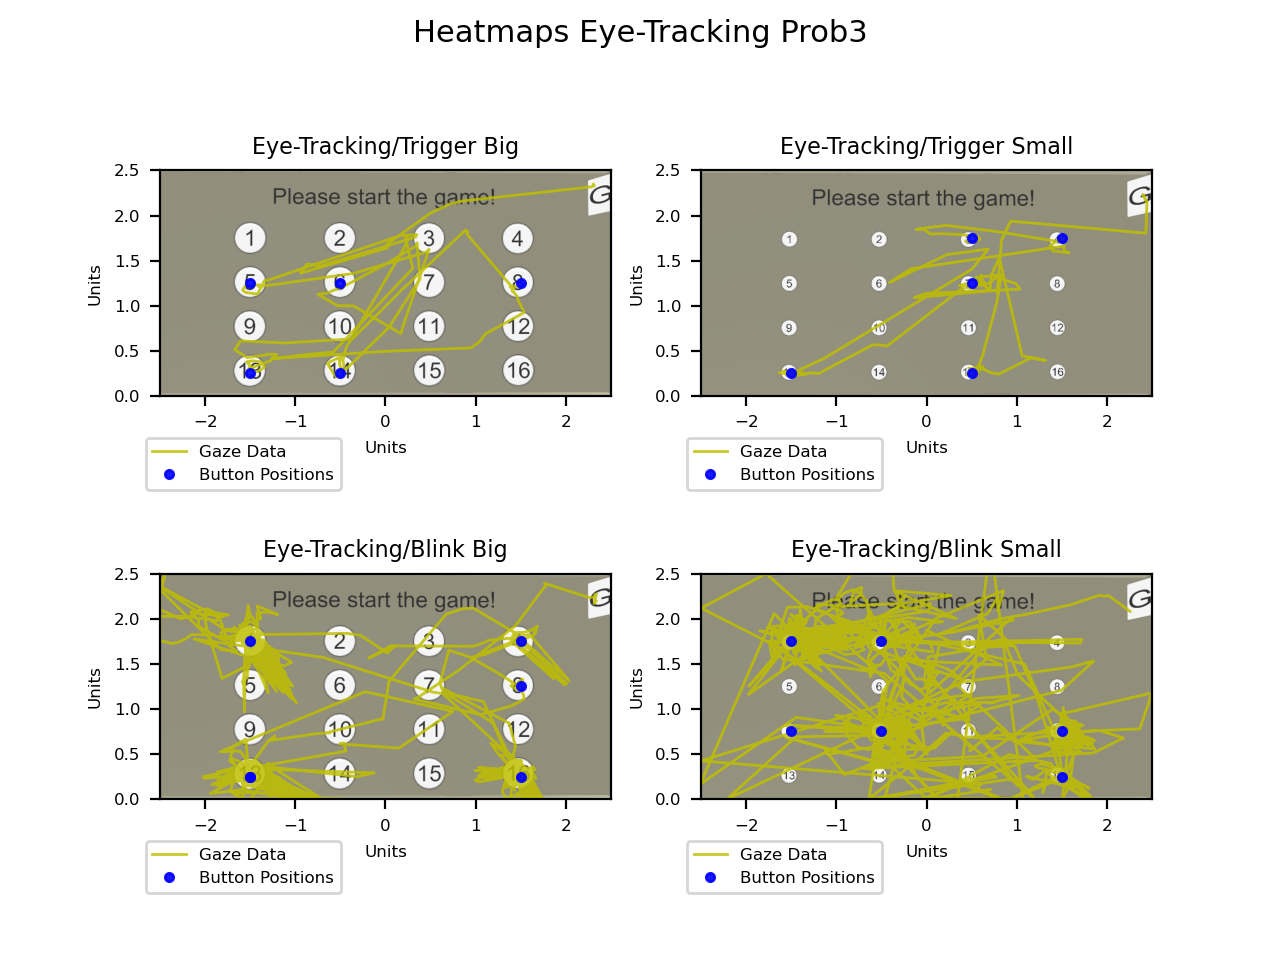
\includegraphics[width=1.0\linewidth]{plot_heatmap_prob3}
	\caption[Visualisierung der Blickdaten und der auszuwählenden Knöpfe] {Visualisierung der Blickdaten und der auszuwählenden Knöpfe}
\end{figure}
\begin{figure}[!htbp]
	\centering
	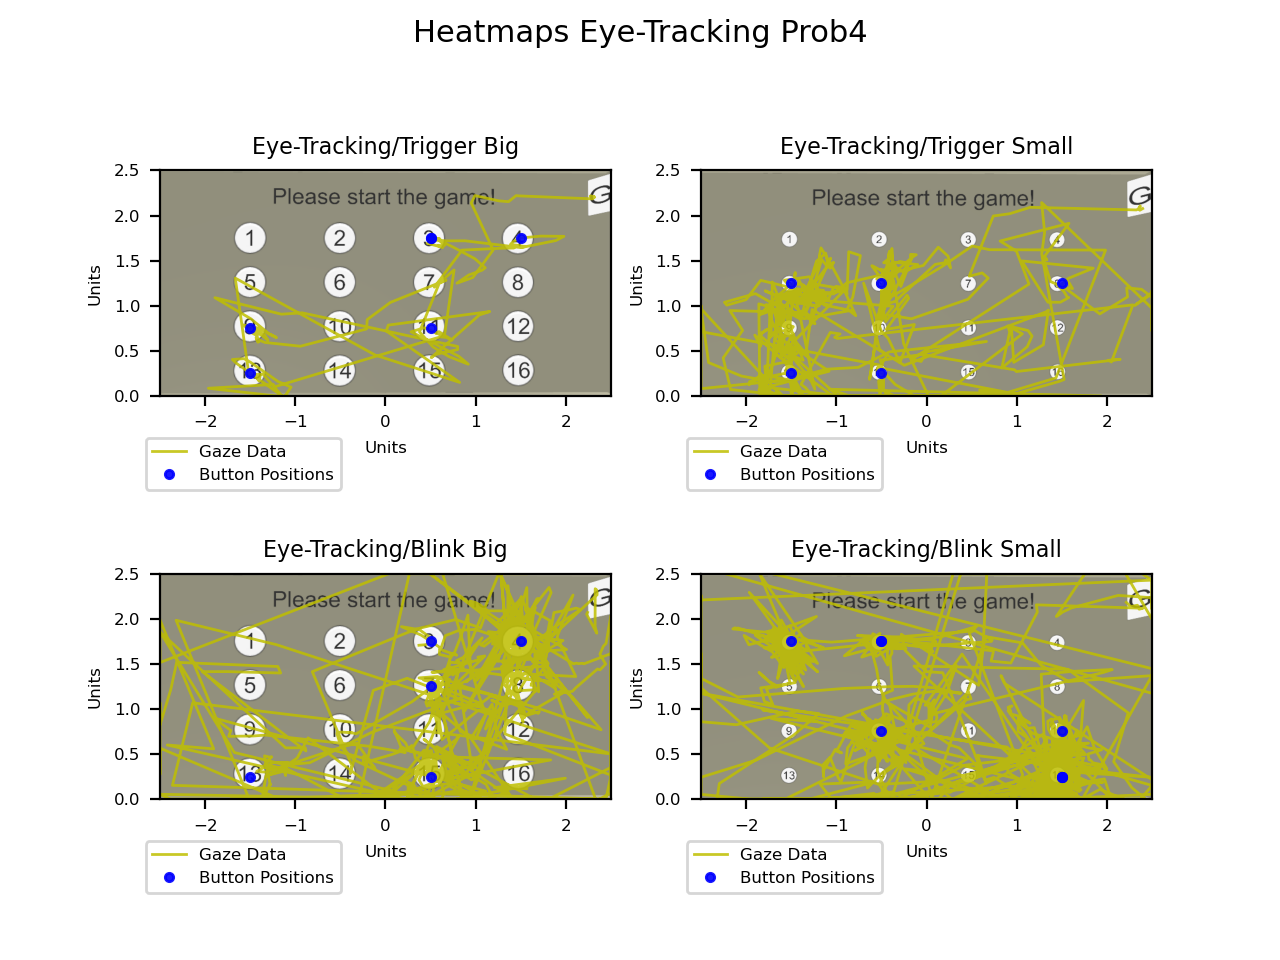
\includegraphics[width=1.0\linewidth]{plot_heatmap_prob4}
	\caption[Visualisierung der Blickdaten und der auszuwählenden Knöpfe] {Visualisierung der Blickdaten und der auszuwählenden Knöpfe}
\end{figure}